\documentclass{ug}
\usepackage{float}
\usepackage{color, colortbl}
\usepackage[section]{placeins}
\usepackage{mathtools}
\usepackage{amsthm}
%\usepackage[T1]{helvet}
\usepackage[OT1]{fontenc} 


\theoremstyle{plain}
\newtheorem*{defn*}{Definition}
\newtheorem*{ex*}{Example}

\definecolor{iob-green}{rgb}{0.0,1.0,0.80}
\definecolor{iob-blue}{rgb}{0.90196,0.94902,1}

\title{IObundle Example User Guide}
\category{User Guide}

\begin{document}
\maketitle
\cleardoublepage
\tableofcontents
\cleardoublepage
\listoftables
\cleardoublepage
\listoffigures
\cleardoublepage


\subsection{Functional Description}
\label{sec:func}

\subsubsection{Hardware Components}


\subsubsection{Software Components}


\section{Interface Signals}

\subsection{General Interface Signals}

\begin{table}[H]
  \begin{center}
    \begin{tabular}{|l|l|p{8cm}|}
      \hline
      \rowcolor{iob-green}
      \textbf{Signal} & \textbf{Direction} & \textbf{Description} \\
      \hline
      \hline

      sys\_clk &  IN & Main system clock \\
      \hline

      \rowcolor{iob-blue} sys\_rst & IN & Asynchronous active high reset
      signal. \\ \hline

      interrupt & OUT & Interrupt signal; goes high if any
      unmasked interrupt bit is high.\\ \hline

    \end{tabular}
    \caption{General interface signals}
    \label{tab:is}
  \end{center}
\end{table}

\subsection{RS232 Interface Signals}

The RS232 IP core used in the {\it Intel FPGA UART Core} described in Chapter 9
of the following document accessed in June/20/2018 from

\hyperlink{https://www.altera.com/en\_US/pdfs/literature/ug/ug\_embedded\_ip.pdf}{https://www.altera.com/en\_US/pdfs/literature/ug/ug\_embedded\_ip.pdf}.

Three instances of this IP are being used, one for each CPU. However, only one
RS232 pin is used, according to the table below:

\begin{table}[H]
  \begin{center}
    \begin{tabular}{|l|l|p{8cm}|}
      \hline
      \rowcolor{iob-green}
      \textbf{Signal} & \textbf{Direction} & \textbf{Description} \\
      \hline
      \hline

      rs232\_tx &  OUT & Serial transmit signal from CPU0\\
      \hline

      rs232\_tx\_1 &  OUT & Serial transmit signal from CPU1\\
      \hline

      rs232\_tx\_2 &  OUT & Serial transmit signal CPU2\\
      \hline

    \end{tabular}
    \caption{RS232 interface signals}
    \label{tab:rs232}
  \end{center}
\end{table}
\clearpage

      
\subsection{SPI Slave Interface}

\begin{table}[H]
  \begin{center}
    \begin{tabular}{|l|l|l|}
      \hline

      \rowcolor{iob-green}
      \textbf{Signal} & \textbf{Direction} & \textbf{Description} \\
      \hline
      \hline

      spi\_sclk & IN & SPI serial (bit) clock.\\ \hline

      \rowcolor{iob-blue} spi\_mosi & IN & SPI master output / slave
      input.\\ \hline

      spi\_miso & OUT & SPI master input / slave output.\\ \hline

      \rowcolor{iob-blue} spi\_ss & IN & SPI slave select. \\ \hline

    \end{tabular}
    \caption{SPI slave interface}
    \label{tab:spi}
  \end{center}
\end{table}

\begin{figure}[H]
  \begin{center}
    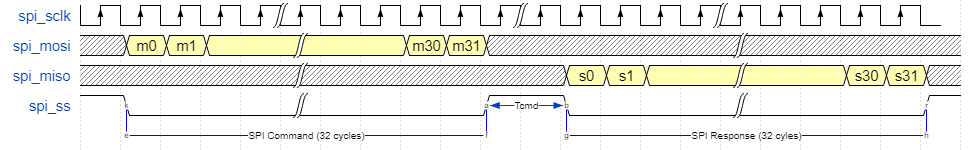
\includegraphics[width=16cm]{spi.png}
    \caption{SPI slave interface timing diagram}
    \label{fig:spi}
  \end{center}
\end{figure}


\begin{table}[H]
\ifnum\XILINX=1
\ifnum\INTEL=1
\begin{minipage}{0.45\linewidth}
\else
\begin{minipage}{\linewidth}
\fi
\centering
\begin{tabular}{|l|r|}
\hline
\rowcolor{iob-green}
\textbf{Resource}  & \textbf{Used} \\
\hline
\hline
\input xil_results.tex 
\end{tabular}
\end{minipage}
\fi
\ifnum\INTEL=1
\ifnum\XILINX=1
\begin{minipage}{0.45\linewidth}
\else
\begin{minipage}{\linewidth}
\fi
\centering
\begin{tabular}{|l|r|}
\hline
\rowcolor{iob-green}
\textbf{Resource}  & \textbf{Used} \\
\hline
\hline
\input alt_results.tex 
\end{tabular}
\end{minipage}
\fi
\ifnum\INTEL=1
\ifnum\XILINX=1
\caption{FPGA results for Kintex Ultrascale (left) and Cyclone V GT (right)}
\fi
\ifnum\XILINX=0
\caption{FPGA results for Cyclone V GT}
\fi
\fi
\ifnum\XILINX=1
\ifnum\INTEL=0
\caption{FPGA results for Kintex Ultrascale}
\fi
\fi
\end{table}



%\bibliographystyle{unsrt}
%\bibliography{rep}
%\nocite{*}

\end{document}
